\section{Debugging}\label{section:prototypische-implementierung:debugging}

\begin{figure}[tbp]
    \centering
    \resizebox{\textwidth}{!}{
        \begin{tikzpicture}
            \begin{class}[text width=7.5cm]{DebuggingAdapterServiceProducer}{0,0}
                \operation{+ sendMessageDAP()}
                \operation{+ onStartSession()}
                \operation{+ onJoinSession()}
                \operation{+ onMessageDAP()}
            \end{class}
            \begin{class}[text width=7.5cm]{DebuggingAdapterServiceConsumer}{8,0}
                \operation{+ sendMessageDAP()}
                \operation{+ startSession()}
                \operation{+ joinSession()}
                \operation{+ onMessageDAP()}
            \end{class}
            \begin{class}[text width=7.5cm]{DebuggingTargetServiceProducer}{0,-3.5}
                \operation{+ sendDebuggingMessage()}
                \operation{+ onStartDebugging()}
                \operation{+ onEndDebugging()}
                \operation{+ onDebuggingMessage()}
            \end{class}
            \begin{class}[text width=7.5cm]{DebuggingTargetServiceConsumer}{8,-3.5}
                \operation{+ sendDebuggingMessage()}
                \operation{+ startDebugging()}
                \operation{+ endDebugging()}
                \operation{+ onDebuggingMessage()}
            \end{class}
        \end{tikzpicture}
    }
    \caption{Klassendiagramm Debugging Services}
    \label{figure:klassendiagramm-debugging-services}
\end{figure}

Für die Bereitstellung der Debug-Funktionen wurde in der prototypischen Implementierung der \textit{\ac{GDB}} \cite{noauthor_gdb_nodate} verwendet. Dieser erlaubt das Debuggen von Microcontrollern und besitzt zudem einen integrierten Debug Adapter. Um \ac{GDB} in Experimenten nutzen zu können, wurde ein cloud-instanziierbares Laborgerät entwickelt. Dieses stellt einen Debugging Adapter Service Producer und einen Debugging Target Service Consumer für die Kommunikation mit der IDE sowie der zu debuggenden Steuereinheit bereit.

In \autoref{figure:klassendiagramm-debugging-services} ist ein Klassendiagramm für den Debugging Adapter Service und den Debugging Target Service dargestellt. Hierbei besitzt der Debugging Adapter Service Consumer die Funktionen \texttt{startSession()} und \texttt{joinSession()}, um eine neue Debug-Sitzung zu starten oder einer laufenden beizutreten. Der Debugging Adapter Service Producer löst entsprechende Events aus, die über Event-Handler behandelt werden können. Sowohl der Debugging Adapter Service Consumer als auch der Debugging Adapter Service Producer besitzen Funktionen, um DAP-Nachrichten zu versenden und auf diese zu reagieren. Der Debugging Target Service Consumer besitzt die Funktionen \texttt{startDebugging()} und \texttt{endDebugging()}, um den Beginn bzw. das Ende einer Debug-Sitzung zu signalisieren. Auch hier löst der Debugging Target Service Producer entsprechende Events aus, die über Event-Handler behandelt werden können. Sowohl der Debugging Target Service Consumer als auch der Debugging Target Service Producer besitzen Funktionen, um Debug-Nachrichten zu versenden und auf diese zu reagieren.

Wenn ein Nutzer eine Debug-Sitzung startet, wird über den Debugging Adapter Service eine entsprechende Nachricht an das Laborgerät des Debuggers gesendet. Diese Nachricht beinhaltet das aktuelle Projekt des Nutzers. Dieses benötigt der Debugger während der Debug-Sitzung, weshalb es für die Dauer der Debug-Sitzung in einem entsprechenden Ordner auf dem Dateisystem hinterlegt wird. Weiterhin wird das Projekt an den Compiler gesendet, wobei für die Ermöglichung des Debuggens spezielle Einstellungen vorgenommen werden müssen. Das Ergebnis der Kompilierung wird dann über den Debugging Target Service an die Steuereinheit gesendet, wodurch der Steuereinheit gleichzeitig der Beginn einer Debug-Sitzung mitgeteilt wird. Weiterhin wird der Debugger selbst gestartet, wobei der tatsächliche Start der Debug-Sitzung erst durch die Nachrichten des \ac{DAP} geschieht. Nachdem alle Vorbereitungen getroffen wurden und eine Antwort von der Steuereinheit empfangen wurde, wird eine Antwort an die IDE gesendet. Die Antwort enthält den Kennzeichner der Debug-Sitzung sowie Einstellungen für diese. Im Falle der prototypischen Implementierung werden hierbei der Kennzeichner der Debug-Sitzung, das Debug-Ziel sowie der Pfad des kompilierten Programms als Einstellungen übergeben. Diese werden dann von der IDE beim Start des \ac{DAP} verwendet.

Damit das \ac{DAP} korrekt ausgeführt werden kann, muss eine Umschreibung der URIs vorgenommen werden, da die Dateien des Nutzers und des Debuggers unterschiedliche URIs besitzen. Außerdem gibt es Dateien, die nur auf dem Dateisystem des Debuggers vorhanden sind, wie z.B. Bibliotheken. Alle URIs, die von der IDE gesendet werden, beginnen entweder mit \texttt{crosslabfs:/workspace} für Dateien innerhalb eines Projekts oder mit \texttt{crosslab-remote:} für Dateien innerhalb des Dateisystems des Debuggers. Bei Ersteren wird das genannte Präfix durch den lokalen Pfad des Projektes auf dem Dateisystem des Debuggers ersetzt, während bei Zweiteren das Präfix gelöscht wird. Bei Nachrichten vom Debugger an die IDE werden Dateien innerhalb des Projekts wieder auf URIs beginnend mit \texttt{crosslabfs:/workspace} abgebildet, während alle anderen Dateien das Präfix \texttt{crosslab-remote:} erhalten.

Um das kollaborative Debuggen innerhalb eines Experiments zu unterstützen, müssen einige Nachrichten des \ac{DAP} speziell behandelt werden. Dazu gehören die Nachrichten für Breakpoints, Stacktraces, das Starten und Stoppen des Programms sowie das Beenden der Debug-Sitzung. Wenn Nutzer einer Debug-Sitzung beitreten, schicken sie zunächst nur ihre lokalen Breakpoints über eine \texttt{SetBreakpoints}-Anfrage. Damit nicht die Breakpoints der anderen Nutzer gelöscht werden, müssen diese entsprechend zu dieser Nachricht hinzugefügt werden. Dafür werden die Breakpoints aller Nutzer separat verwaltet. Außerdem müssen alle Events gespeichert werden, um diese beitretenden Nutzern schicken und den aktuellen Zustand der Debug-Sitzung herstellen zu können. Allgemein werden Events, die vom Debug Adapter ausgegeben werden, an alle Nutzer einer Debug-Sitzung gesendet. Wenn ein Nutzer das Programm startet oder fortsetzt, muss ein \texttt{Continued}-Event an die anderen Nutzer gesendet werden. Bei Breakpoints und Stacktraces muss darauf geachtet werden, dass die URIs für Dateien des Debuggers entsprechend angepasst werden, damit die IDE diese öffnen kann. Wenn der Ersteller der Debug-Sitzung diese beendet, so wird sie für alle Nutzer beendet. Sollte ein anderer Nutzer die Debug-Sitzung beenden, so wird sie nur für diesen Nutzer selbst beendet.

\begin{figure}[tbp]
    \centering
    \begin{tikzpicture}
        \node[anchor=south west,inner sep=0] at (0,0) {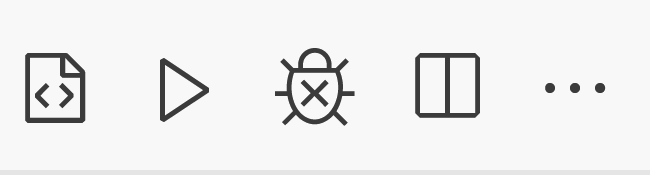
\includegraphics[trim={8.5cm 0 9.1cm 0},clip,width=0.1\textwidth]{images/symbols.png}};
        \node[anchor=south west,inner sep=0] at (2,0) {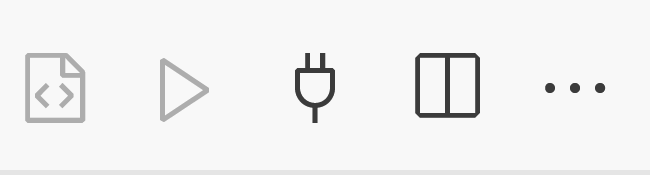
\includegraphics[trim={8.5cm 0 9.1cm 0},clip,width=0.1\textwidth]{images/symbols-join.png}};
        \draw[orange,ultra thick,rounded corners] (0.2,0.2) rectangle (1.35,1.55);
        \draw[blue!60,ultra thick,rounded corners] (2.2,0.2) rectangle (3.35,1.55);
        \node[orange] at (-2.8,0.75) {Starten einer Debug-Sitzung};
        \node[blue!60] at (6.5,0.75) {Beitreten einer Debug-Sitzung};
    \end{tikzpicture}
    \caption{Schaltflächen für das Starten und Beitreten einer Debug-Sitzung}
    \label{figure:benutzerinterface:symbole-debugging}
\end{figure}

\begin{figure}[tbp]
    \centering
    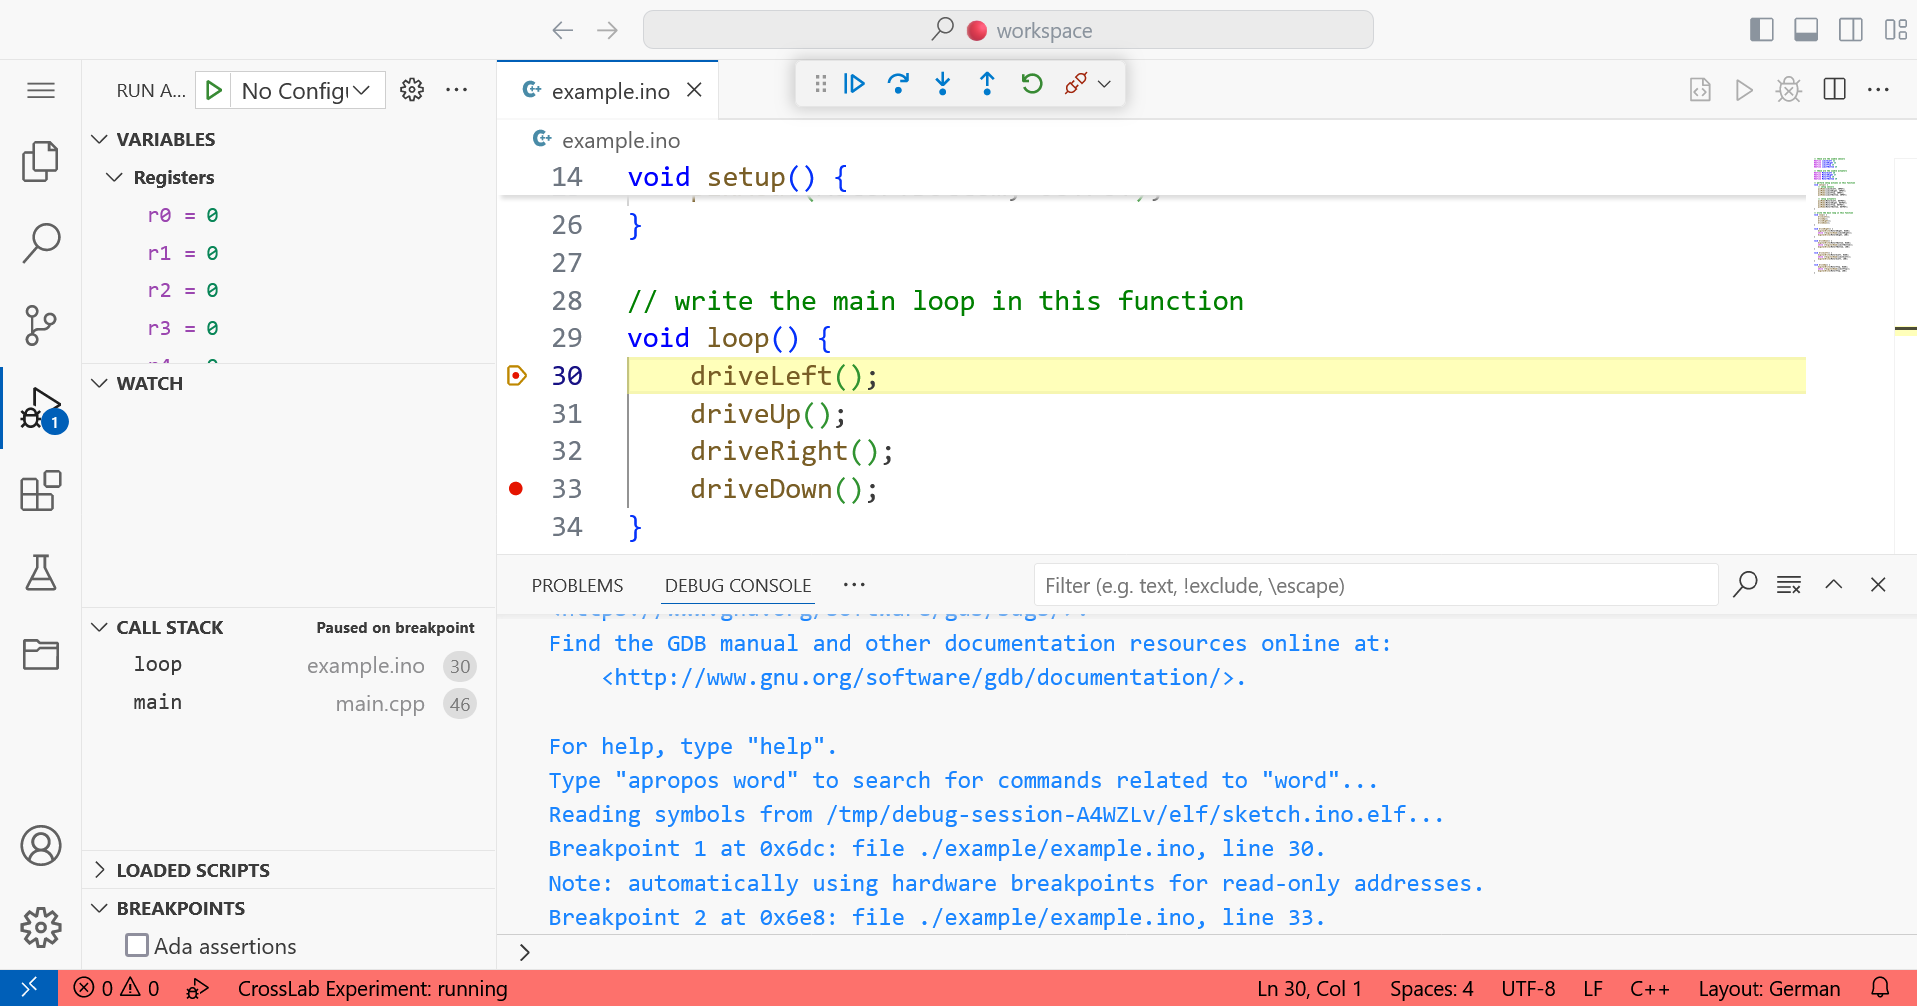
\includegraphics[trim={0 3px 0 0},clip,width=\textwidth]{images/debugging.png}
    \caption{Benutzerinterface der IDE während einer aktiven Debug-Sitzung}
    \label{figure:benutzerinterface:debugging}
\end{figure}

Für die Einbindung in die IDE wurde eine entsprechende Erweiterung entwickelt. Diese wird im Folgenden als \textit{Debugging Erweiterung} bezeichnet und fügt einen Debugging Adapter Service Consumer hinzu. Die Debugging Erweiterung beinhaltet zudem Implementierungen der Schnittstellen \texttt{DebugAdapter}, \texttt{DebugAdapterDescriptorFactory} und \texttt{DebugConfigurationProvider}. Mithilfe dieser Schnittstellen kann bereits ein Großteil der Funktionalität implementiert werden. Weiterhin werden auch Bedienelemente zum Starten bzw. Beitreten einer Debug-Sitzung bereitgestellt. Diese sind in \autoref{figure:benutzerinterface:symbole-debugging} dargestellt. Nutzer können eine Debug-Sitzung über eine entsprechende Schaltfläche starten, falls keine aktive Debug-Sitzung bestehen sollte. Ansonsten können Nutzer über eine weitere Schaltfläche einer bestehenden Debug-Sitzung beitreten, falls sie Zugriff auf das dazugehörige Projekt haben. In \autoref{figure:benutzerinterface:debugging} wird das Benutzerinterface der IDE während einer aktiven Debug-Sitzung gezeigt. Um das Debuggen von Dateien zu ermöglichen, die nur im Dateisystem des Debuggers vorhanden sind, wurde ein \texttt{TextDocumentContentProvider} implementiert. Dieser ermöglicht Lesezugriff auf die Dateien innerhalb des Dateisystems des Debuggers sowie das Setzen von Breakpoints innerhalb dieser.

Das betrachtete Experiment wird um das neue Laborgerät für die Bereitstellung von GDB erweitert. Dieses wird über den Debugging Adapter Service mit den IDEs verbunden. Außerdem wird die Steuereinheit um einen Debugging Target Service Producer erweitert. Der Debugger wird über den Debugging Target Service mit der Steuereinheit verbunden (siehe \autoref{figure:experimentkonfiguration:debugging}).